\documentclass[11pt,a4paper]{article}
\usepackage[utf8]{inputenc}
\usepackage[T1]{fontenc}
\usepackage{amsmath,amssymb,amsfonts}
\usepackage{amsthm}
\usepackage[margin=2.5cm]{geometry}
\usepackage{enumitem}
\usepackage{tikz}
\usepackage{xcolor}
\usepackage{hyperref}
\hypersetup{colorlinks=true,linkcolor=blue!55!black,urlcolor=blue!55!black}
\setlist[itemize]{leftmargin=1.4em,itemsep=2pt,topsep=3pt}

% ── theorem environments (numbered, standard) ──
\newtheorem{theorem}{Theorem}[section]
\newtheorem{lemma}[theorem]{Lemma}
\newtheorem{proposition}[theorem]{Proposition}
\newtheorem{corollary}[theorem]{Corollary}
\theoremstyle{definition}
\newtheorem{definition}[theorem]{Definition}
\newtheorem{example}[theorem]{Example}
\newtheorem{remark}[theorem]{Remark}
\newtheorem{exercise}{Exercise}

% ── master macro block (safe, multi-character) ──
\newcommand{\Z}{\mathbb{Z}}
\newcommand{\Q}{\mathbb{Q}}
\newcommand{\R}{\mathbb{R}}
\newcommand{\C}{\mathbb{C}}
\newcommand{\F}{\mathbb{F}}
\newcommand{\N}{\mathbb{N}}
\newcommand{\id}{\operatorname{id}}
\newcommand{\ch}{\operatorname{char}}
\newcommand{\Gal}{\operatorname{Gal}}
\newcommand{\Aut}{\operatorname{Aut}}
\newcommand{\ord}{\operatorname{ord}}
\newcommand{\Spec}{\operatorname{Spec}}

\title{
  {\color{blue!40!black}\textbf{\Huge Point}}\\[0.3em]
  \Large \textit{From Number Theory to Algebraic Geometry and Logic}\\[0.7em]
  \large \textbf{Session S3 --- Fields, Extensions, and Algebraic Closure}\\[0.3em]
  \normalsize \emph{Complete lecture notes with proofs, examples, and exercises}
}
\author{}
\date{}

\begin{document}
\maketitle
\thispagestyle{empty}

\begin{abstract}
\noindent
This session builds the \emph{arenas} in which the course's points live: fields and their
extensions. A field is where polynomials have (or fail to have) roots --- i.e.\ where algebraic
points exist; an extension $L/K$ measures how many new points appear; the minimal polynomial is
the equation that cuts a point out; and the algebraic closure $\bar K$ is the space of \emph{all}
algebraic points over $K$, whose symmetry group $\Gal(\bar K/K)$ --- for $K=\Q$ the group $G_\Q$ ---
is the horizon of the entire course (S16, S35, S45). Everything is proved from the ring theory of
S1: Krull's theorem (via Zorn) is exactly what makes algebraic closures exist.
\end{abstract}

\subsection*{Session plan (150 minutes)}
\begin{center}\small
\begin{tabular}{|l|l|}
\hline
\textbf{Time} & \textbf{Block} \\
\hline
0:00--0:10 & Orientation: fields as arenas of points; where S3 feeds (S12--S16, S20, S45) \\
0:10--0:35 & \S1 Fields, characteristic, prime subfields, finite fields \\
0:35--1:05 & \S2 Extensions, degree, tower law, minimal polynomials, simple extensions \\
1:05--1:15 & \emph{Break} \\
1:15--1:45 & \S3 Algebraic closure: existence via Zorn (S1), uniqueness, $\bar\Q$ vs $\C$ \\
1:45--2:10 & \S4 Preview: $\Gal(L/K)$, the group $G_\Q$, profinite horizon (S16, S34) \\
2:10--2:30 & Exercises / wrap-up: algebraic closure $=$ space of all algebraic points \\
\hline
\end{tabular}
\end{center}

\subsection*{Conventions}
All fields are commutative with $1\neq0$. An \emph{extension} $L/K$ means $K\subseteq L$ with the
same operations; we write $[L:K]$ for its degree. $K[x]$ denotes the polynomial ring and $K(x)$
the field of rational functions. By S1, every nonzero ring has a maximal ideal (Krull, via Zorn) ---
this is used essentially in \S3.

\tableofcontents
\newpage

% ══════════════════════════════════════════════
\section{Fields, Characteristic, and Finite Fields}
% ══════════════════════════════════════════════

\begin{definition}[Field]
A \textbf{field} is a commutative ring $K$ with $1\neq0$ in which every $a\neq0$ has a multiplicative
inverse $a^{-1}$. Equivalently: the only ideals of $K$ are $0$ and $K$ (S1).
\end{definition}

\begin{example}[Fields old and new]\label{ex:fields}
\begin{itemize}
  \item $\Q$, $\R$, $\C$; the $p$-adic fields $\Q_p$ (S18); function fields $k(x)$ (S21).
  \item $\F_p=\Z/p\Z$ for prime $p$ (a field because $(p)$ is maximal, S1).
  \item $K=\Q(\sqrt2)=\{a+b\sqrt2:a,b\in\Q\}$ --- a first ``point-adding'' extension (\S2).
  \item Non-examples: $\Z$, $\Z/n\Z$ for composite $n$, $k[x]$ (ideals $(x)$, $(x^2)$ are proper and nonzero).
\end{itemize}
\end{example}

\begin{definition}[Characteristic]
The \textbf{characteristic} $\ch(K)$ is the smallest $n\ge1$ with $\underbrace{1+\cdots+1}_{n}=0$;
if no such $n$ exists, $\ch(K)=0$.
\end{definition}

\begin{proposition}[Characteristic is $0$ or prime]\label{prop:char}
$\ch(K)\in\{0\}\cup\{\text{primes}\}$.
\end{proposition}
\begin{proof}
If $\ch(K)=n=ab$ with $1<a,b<n$, then $0=n\cdot1=(a\cdot1)(b\cdot1)$; a field has no zero-divisors,
so $a\cdot1=0$ or $b\cdot1=0$, contradicting minimality of $n$.
\end{proof}

\begin{proposition}[Prime subfield]\label{prop:prime-subfield}
The intersection of all subfields of $K$ is a subfield, the \textbf{prime subfield}, isomorphic to
$\Q$ if $\ch(K)=0$ and to $\F_p$ if $\ch(K)=p$.
\end{proposition}
\begin{proof}
The unique ring map $\varphi:\Z\to K$, $n\mapsto n\cdot1$, has kernel $(\ch K)$ by definition; if
$\ch K=p$ then $\varphi$ descends to an embedding $\F_p\hookrightarrow K$; if $\ch K=0$ then
$\varphi$ extends to an embedding $\Q\hookrightarrow K$ (universal property of localization, S1/S2).
Any subfield contains $1$, hence the image; so the image is the smallest subfield.
\end{proof}

\begin{proposition}[Order of a finite field]\label{prop:ff-order}
If $|K|<\infty$ then $|K|=p^n$ where $p=\ch(K)$ and $n=[K:\F_p]$.
\end{proposition}
\begin{proof}
$\ch(K)=p>0$ else $\Q\subseteq K$ would be infinite (Proposition~\ref{prop:prime-subfield}).
Then $K$ is an $\F_p$-vector space; finiteness forces finite dimension $n$, and counting gives
$|K|=p^n$.
\end{proof}

\begin{proposition}[Finite multiplicative subgroups are cyclic]\label{prop:finite-cyclic}
Every finite subgroup $G\subseteq K^\times$ of a field is cyclic. In particular
$(\Z/p)^\times$ and $\F_q^\times$ are cyclic (the primitive-root engine of S5).
\end{proposition}
\begin{proof}
Let $m=|G|$ and let $e$ be the exponent of $G$ (lcm of element orders). Every $g\in G$ is a root of
$x^e-1$, which has at most $e$ roots in $K$; since $G$ supplies $m$ distinct roots, $m\le e$. Always
$e\mid m$... more precisely $e\le m$ and $m\mid e$? Standard finish: $e\le m$ by the root bound and
$m\le e$ since some element realizes... cleanly: the root bound gives $m\le e$; Lagrange (P1) gives
$\ord(g)\mid m$ for all $g$, hence $e\mid m$, so $e=m$. An element of order $e=m$ exists (else the
exponent of a proper... ) --- take $g$ with $\ord(g)=e$: exists because $e$ is an lcm of orders and
in an abelian group orders compose: if $\ord(a)=r$, $\ord(b)=s$ then some element has order
$\operatorname{lcm}(r,s)$ (write $r=r_1r_2$ coprime pieces); hence some $g$ has order $e=m$ and
$G=\langle g\rangle$.
\end{proof}

\begin{remark}[What is postponed to S12]
Existence and uniqueness of a field $\F_{p^n}$ for each $p,n$ (as the splitting field of
$x^{p^n}-x$), and the lattice of subfields $\F_{p^d}$, $d\mid n$, are proved in S12 together with
the Frobenius automorphism --- the first canonical ``point-moving'' symmetry of the course.
\end{remark}

% ══════════════════════════════════════════════
\section{Extensions, Degree, and Minimal Polynomials}
% ══════════════════════════════════════════════

\begin{definition}[Extension and degree]
An \textbf{extension} $L/K$ is a field $L$ containing $K$. Then $L$ is a $K$-vector space; its
dimension is the \textbf{degree} $[L:K]$. The extension is \textbf{finite} if $[L:K]<\infty$.
\end{definition}

\begin{example}\label{ex:degrees}
\begin{itemize}
  \item $[\C:\R]=2$ with basis $\{1,i\}$; $[\Q(\sqrt2):\Q]=2$ with basis $\{1,\sqrt2\}$.
  \item $[\R:\Q]=\infty$ (else $\R$ would be countable --- it is not).
  \item $[K(x):K]=\infty$: $1,x,x^2,\dots$ are linearly independent.
\end{itemize}
\end{example}

\begin{proposition}[Tower law]\label{prop:tower}
If $K\subseteq M\subseteq L$ then $[L:K]=[L:M]\,[M:K]$ (with the convention $\infty\cdot n=\infty$).
\end{proposition}
\begin{proof}
Let $\{m_i\}_{i\in I}$ be a $K$-basis of $M$ and $\{l_j\}_{j\in J}$ an $M$-basis of $L$. Then
$\{m_i l_j\}_{(i,j)\in I\times J}$ is a $K$-basis of $L$: spanning --- any $x=\sum_j a_j l_j$ with
$a_j=\sum_i c_{ij} m_i$; independence --- if $\sum_{i,j} c_{ij} m_i l_j=0$ then
$\sum_i c_{ij}m_i=0$ for each $j$ (independence of the $l_j$ over $M$), hence all $c_{ij}=0$.
Counting gives the formula.
\end{proof}

\begin{definition}[Algebraic and transcendental elements]
$\alpha\in L$ is \textbf{algebraic over $K$} if $f(\alpha)=0$ for some nonzero $f\in K[x]$;
otherwise \textbf{transcendental}. $L/K$ is \textbf{algebraic} if every $\alpha\in L$ is algebraic.
\end{definition}

\begin{proposition}[Minimal polynomial and simple extensions]\label{prop:minpoly}
Let $\alpha\in L$. The evaluation map $\operatorname{ev}_\alpha:K[x]\to L$, $f\mapsto f(\alpha)$, is a
ring homomorphism with kernel an ideal of the PID $K[x]$.
\begin{enumerate}[label=(\alph*)]
  \item If $\ker=0$ then $\alpha$ is transcendental and $K(\alpha)\cong K(x)$, $[K(\alpha):K]=\infty$.
  \item If $\ker\neq0$ then $\ker=(m_\alpha)$ for a unique monic irreducible $m_\alpha$, the
    \textbf{minimal polynomial} of $\alpha$; then $K(\alpha)=K[\alpha]\cong K[x]/(m_\alpha)$ and
    $[K(\alpha):K]=\deg m_\alpha$, with basis $1,\alpha,\dots,\alpha^{d-1}$, $d=\deg m_\alpha$.
\end{enumerate}
\end{proposition}
\begin{proof}
$K[x]$ is a PID (S1: Euclidean domain). In case (b), $\ker$ is a nonzero prime ideal (kernel of a
map into a field), hence maximal in a PID, so $K[x]/(m_\alpha)$ is a field containing $K$ and
$\alpha$, hence equal to $K(\alpha)$; the cosets of $1,x,\dots,x^{d-1}$ give the claimed basis by
Euclidean division. Uniqueness of the monic generator is immediate.
\end{proof}

\begin{example}\label{ex:minpoly}
\begin{itemize}
  \item $m_{\sqrt2,\Q}=x^2-2$; $m_{\sqrt[3]{2},\Q}=x^3-2$ (irreducible by Eisenstein, or degree-3
    root test); $m_{i,\R}=x^2+1$.
  \item $\alpha=\sqrt2+\sqrt3$: $\alpha^2=5+2\sqrt6$, $(\alpha^2-5)^2=24$, so
    $m_{\alpha,\Q}=x^4-10x^2+1$; hence $[\Q(\sqrt2+\sqrt3):\Q]=4$, and since
    $\Q(\sqrt2+\sqrt3)\subseteq\Q(\sqrt2,\sqrt3)$ with $[\Q(\sqrt2,\sqrt3):\Q]\le4$ (tower law),
    equality holds: $\Q(\sqrt2,\sqrt3)=\Q(\sqrt2+\sqrt3)$ --- a primitive element (preview of S12).
  \item $\pi$ is transcendental over $\Q$ (Lindemann--Weierstrass; out of scope) so
    $[\Q(\pi):\Q]=\infty$.
\end{itemize}
\end{example}

\begin{proposition}[Finite $\Rightarrow$ algebraic; f.g.\ algebraic $\Rightarrow$ finite]\label{prop:fin-alg}
\begin{enumerate}[label=(\alph*)]
  \item If $[L:K]<\infty$ then $L/K$ is algebraic.
  \item If $L=K(\alpha_1,\dots,\alpha_r)$ with all $\alpha_i$ algebraic over $K$, then $[L:K]<\infty$.
\end{enumerate}
\end{proposition}
\begin{proof}
(a) For $\alpha\in L$, the vectors $1,\alpha,\dots,\alpha^{[L:K]}$ are linearly dependent, giving a
nonzero annihilating polynomial. (b) Induction on $r$ with the tower law: each step
$K(\alpha_1,\dots,\alpha_i)$ over $K(\alpha_1,\dots,\alpha_{i-1})$ is finite because $\alpha_i$ is
algebraic over $K$, hence over the larger field (its minimal polynomial over $K$ still annihilates
it), so Proposition~\ref{prop:minpoly}(b) bounds the degree.
\end{proof}

\begin{corollary}[Algebraic elements form a field]\label{cor:alg-closure-in-L}
For $K\subseteq L$, the set $\{\alpha\in L:\alpha\text{ algebraic over }K\}$ is a subfield of $L$
(the \textbf{algebraic closure of $K$ in $L$}).
\end{corollary}
\begin{proof}
For algebraic $\alpha,\beta\neq0$, the extension $K(\alpha,\beta)$ is finite
(Proposition~\ref{prop:fin-alg}(b)), hence algebraic (part (a)); and
$\alpha\pm\beta,\ \alpha\beta,\ \alpha^{-1}\in K(\alpha,\beta)$, so all are algebraic.
\end{proof}

\begin{figure}[h]
\centering
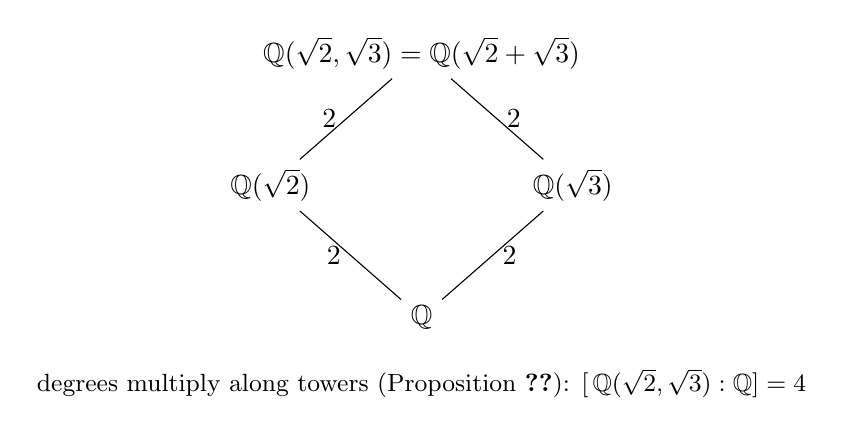
\begin{tikzpicture}[scale=1.2]
  \node (Q) at (0,0) {$\Q$};
  \node (A) at (-1.6,1.4) {$\Q(\sqrt2)$};
  \node (B) at (1.6,1.4) {$\Q(\sqrt3)$};
  \node (T) at (0,2.8) {$\Q(\sqrt2,\sqrt3)=\Q(\sqrt2+\sqrt3)$};
  \draw (Q) -- node[left] {$2$} (A);
  \draw (Q) -- node[right] {$2$} (B);
  \draw (A) -- node[left] {$2$} (T);
  \draw (B) -- node[right] {$2$} (T);
  \node at (0,-0.7) {\small degrees multiply along towers (Proposition~\ref{prop:tower}): $[\,\Q(\sqrt2,\sqrt3):\Q]=4$};
\end{tikzpicture}
\caption{A tower of simple extensions: each step adds one algebraic point, and degrees multiply.}
\end{figure}

% ══════════════════════════════════════════════
\section{Algebraic Closure: Existence and Uniqueness}
% ══════════════════════════════════════════════

\begin{definition}[Algebraically closed; algebraic closure]
$L$ is \textbf{algebraically closed} if every non-constant $f\in L[x]$ has a root in $L$
(equivalently: splits into linear factors; equivalently: $L$ has no proper algebraic extension).
An \textbf{algebraic closure} of $K$ is a field $\bar K$ that is algebraically closed and algebraic
over $K$.
\end{definition}

\begin{theorem}[Existence of algebraic closures (Artin)]\label{thm:alg-closure}
Every field $K$ has an algebraic closure.
\end{theorem}
\begin{proof}
\emph{Step 1 (one root for everything at once).} Let $S$ be the set of monic irreducible polynomials
of $K[x]$ and $R=K[x_f:f\in S]$ the polynomial ring in one variable per $f$. Let
$I=(f(x_f):f\in S)\subseteq R$. Then $1\notin I$: any relation $1=\sum_{i=1}^r g_i f_i(x_{f_i})$
lives in the subring $K[x_{f_1},\dots,x_{f_r}]$, and the quotient of that subring by
$(f_1(x_1),\dots,f_r(x_r))$ is $K[x]/(f_1)\otimes_K\cdots\otimes_K K[x]/(f_r)$, a tensor product of
fields, hence nonzero (S2), so $1$ cannot lie in the ideal. By Krull's theorem (S1, via Zorn) extend
$I$ to a maximal ideal $M$; then $L_1:=R/M$ is a field containing $K$ in which every $f\in S$ ---
hence every non-constant $f\in K[x]$ --- has a root (the image of $x_f$).

\emph{Step 2 (iterate).} Apply Step 1 repeatedly: $K\subseteq L_1\subseteq L_2\subseteq\cdots$ with
every non-constant polynomial over $L_i$ having a root in $L_{i+1}$. Set $L=\bigcup_i L_i$ (a field:
operations land in some stage). Every non-constant $f\in L[x]$ has coefficients in some $L_i$, hence
a root in $L_{i+1}\subseteq L$; a field in which every non-constant polynomial has a root is
algebraically closed (factor out the root and induct on degree).

\emph{Step 3 (cut to algebraic part).} Let $\bar K=\{\alpha\in L:\alpha\text{ algebraic over }K\}$;
this is a field by Corollary~\ref{cor:alg-closure-in-L}, algebraic over $K$ by construction, and
algebraically closed: any non-constant $f\in\bar K[x]$ has a root $\beta\in L$; $\beta$ is algebraic
over $\bar K$, hence over $K$ (tower of algebraic extensions, Proposition~\ref{prop:fin-alg}), so
$\beta\in\bar K$. Thus $\bar K$ is an algebraic closure of $K$.
\end{proof}

\begin{theorem}[Uniqueness of algebraic closures]\label{thm:alg-closure-unique}
Any two algebraic closures of $K$ are isomorphic over $K$ (by an isomorphism fixing $K$ pointwise).
\end{theorem}
\begin{proof}[Proof idea]
Consider the set of pairs $(M,\varphi)$ with $K\subseteq M\subseteq\bar K_1$ an intermediate field and
$\varphi:M\to\bar K_2$ a $K$-embedding; order by extension. Zorn (S1) gives a maximal $(M,\varphi)$.
If $M\neq\bar K_1$, pick $\alpha\in\bar K_1\setminus M$ with minimal polynomial $m$ over $M$;
$\varphi(m)$ has a root $\beta$ in $\bar K_2$ (algebraically closed), and $\varphi$ extends to
$M(\alpha)\cong M[x]/(m)\to\bar K_2$, $x\mapsto\beta$ --- contradicting maximality. Hence
$M=\bar K_1$; then $\varphi(\bar K_1)$ is algebraically closed inside $\bar K_2$ and contains $K$,
so equals $\bar K_2$ (algebraicity), i.e.\ $\varphi$ is an isomorphism.
\end{proof}

\begin{example}[$\bar\Q$ versus $\C$]\label{ex:Qbar}
\begin{itemize}
  \item $\bar\Q$ is \textbf{countable}: it is the union over all $f\in\Q[x]$ (countably many) of the
    finite root sets of $f$.
  \item $\C$ is \textbf{uncountable} (Cantor's diagonal); hence $\bar\Q\subsetneq\C$, and
    $e,\pi\in\C\setminus\bar\Q$ are transcendental.
  \item $\bar\Q$ is not complete for $|\cdot|$ (its completion is $\C$? no --- the completion of
    $\bar\Q$ for $|\cdot|$ is $\C$; the completion of $\Q$ is $\R$, P2); for each $p$, the completion
    of $\bar\Q$ for $|\cdot|_p$ is $\C_p$ (S18--S19). Closures add \emph{algebraic} points;
    completions add \emph{limit} points --- the two machines of the course, side by side.
\end{itemize}
\end{example}

% ══════════════════════════════════════════════
\section[Preview: Galois Groups and the Horizon of the Course]{Preview: Galois Groups and the Horizon $G_\Q$}
% ══════════════════════════════════════════════

\begin{definition}[Galois group of an extension, preview]
For $L/K$, write $\Aut(L/K)$ for the group of field automorphisms of $L$ fixing $K$ pointwise.
When $L/K$ is finite and \emph{Galois} (separable + normal, S12), this group has order $[L:K]$ and
controls all intermediate fields (FTGT, S13).
\end{definition}

\begin{example}[First computations]\label{ex:first-galois}
\begin{itemize}
  \item $\Aut(\Q(\sqrt2)/\Q)=\{\id,\ \sqrt2\mapsto-\sqrt2\}\cong\Z/2$: the two roots of $x^2-2$ are the
    two ``positions'' of the point $\sqrt2$, and the group permutes them.
  \item $\Aut(\C/\R)=\{\id,\text{conjugation}\}\cong\Z/2$.
  \item $\Aut(\F_{p^n}/\F_p)$ is generated by the Frobenius $x\mapsto x^p$ (S12).
\end{itemize}
\end{example}

\begin{definition}[The absolute Galois group]
$G_K:=\Gal(\bar K/K):=\Aut(\bar K/K)$, equipped with the Krull/profinite topology as an inverse
limit of the finite groups $\Gal(L/K)$ over finite Galois subextensions $L/K$ (S16, S34). For
$K=\Q$ this is $G_\Q$ --- the symmetry group of \emph{all} algebraic points of $\Q$.
\end{definition}

\begin{remark}[Why $G_\Q$ is the horizon of the course]
Class field theory (Act VI) computes the abelianization $G_\Q^{\mathrm{ab}}$ completely
(Kronecker--Weber, S16/S47--S49); the \'etale fundamental group (S35) identifies $G_K$ with
$\pi_1^{\text{\'et}}(\Spec K)$, making Galois theory a special case of topology-of-schemes;
Galois cohomology (S45) measures its failure to be trivial; and Deligne's theorem (S58) is the
logical shadow of ``enough points''. Everything grows from the single object $\bar K$ built in
Theorem~\ref{thm:alg-closure}.
\end{remark}

% ══════════════════════════════════════════════
\section{Exercises}
% ══════════════════════════════════════════════
\begin{exercise}
Prove Proposition~\ref{prop:char} and Proposition~\ref{prop:prime-subfield} in full detail, and
identify the prime subfield of $\F_{p^n}$, $\Q_p$, and $\C$.
\end{exercise}
\begin{exercise}
Fill in the abelian-group lemma used in Proposition~\ref{prop:finite-cyclic}: if $\ord(a)=r$ and
$\ord(b)=s$ in an abelian group, some element has order $\operatorname{lcm}(r,s)$. Conclude that
$\F_q^\times$ is cyclic.
\end{exercise}
\begin{exercise}
Using the tower law (Proposition~\ref{prop:tower}), compute $[\Q(\sqrt2,\sqrt3):\Q]$ by exhibiting
an explicit basis; then verify $\Q(\sqrt2,\sqrt3)=\Q(\sqrt2+\sqrt3)$ as in Example~\ref{ex:minpoly}.
\end{exercise}
\begin{exercise}
Find the minimal polynomials over $\Q$ of: $\sqrt3+\sqrt5$; $\sqrt[3]{2}+1$; $i\sqrt2$; and
$\cos(2\pi/5)$ (hint: $\zeta_5+\zeta_5^{-1}$; cyclotomics appear in S9).
\end{exercise}
\begin{exercise}
Show that $\bar\Q/\Q$ is algebraic but $[\bar\Q:\Q]=\infty$ (consider $\sqrt[n]{2}$ for all $n$).
Conclude that the converse of Proposition~\ref{prop:fin-alg}(a) fails.
\end{exercise}
\begin{exercise}
Prove that for algebraic $\alpha$ over $K$, $K(\alpha)=K[\alpha]$ (every element is a polynomial in
$\alpha$), and compute the inverse of $1+\sqrt2+\sqrt3$ inside $\Q(\sqrt2,\sqrt3)$ explicitly.
\end{exercise}
\begin{exercise}
In Step 1 of Theorem~\ref{thm:alg-closure}, prove carefully that
$K[x]/(f_1)\otimes_K\cdots\otimes_K K[x]/(f_r)\neq0$ using only S2 (tensor products of free
modules, base change) --- this is exactly where the linear layer of S2 earns its keep.
\end{exercise}
\begin{exercise}
Show that a field $L$ in which every non-constant polynomial has a root is algebraically closed
(induction on degree, factoring out roots).
\end{exercise}
\begin{exercise}
Prove that $\bar\Q$ is countable while $\C$ is not; deduce the existence of transcendentals without
naming any. Then show $\Q(\pi)\cong\Q(x)$ (rational function field).
\end{exercise}
\begin{exercise}
Compute $\Aut(\Q(\sqrt2,\sqrt3)/\Q)$ explicitly (four automorphisms; identify the group as
$\Z/2\times\Z/2$) and match each automorphism to a choice of signs for $(\sqrt2,\sqrt3)$ ---
a first taste of the FTGT dictionary (S13).
\end{exercise}
\begin{exercise}
Show that any finite subgroup of $\Aut(L/K)$ has order at most $[L:K]$ (hint: linear independence of
characters --- Dedekind's lemma, proved in S12; accept it here as a black box if you prefer).
\end{exercise}

% ══════════════════════════════════════════════
\section*{Where This Session Feeds the Course}
\addcontentsline{toc}{section}{Where This Session Feeds the Course}
% ══════════════════════════════════════════════
\begin{itemize}
  \item \textbf{Depends on:} S1 (PID structure of $K[x]$, Krull/Zorn), S2 (tensor products in
    Step 1 of Theorem~\ref{thm:alg-closure}), P1 (Lagrange, cyclic groups).
  \item \textbf{Feeds:} S12--S16 (Galois theory, finite fields, $G_\Q$); S20 (degrees $e,f$ of
    valuation extensions); S38 (Riemann surfaces over $\C$); S45 (Galois cohomology of $G_K$);
    S50 (Lubin--Tate over $\Q_p$).
  \item \textbf{Unifying thread:} a field is an arena of points (roots); an extension adds points;
    the minimal polynomial is the equation of a point; the algebraic closure $\bar K$ is the space
    of \emph{all} algebraic points, and $G_K=\Aut(\bar K/K)$ is the group permuting them ---
    evaluation and symmetry, unified.
\end{itemize}

\subsection*{References for this session}
\begin{enumerate}[label={[\arabic*]}]
  \item Lang, S. \emph{Algebra}, ch.V (extensions, algebraic closures).
  \item Artin, E. \emph{Galois Theory}, ch.1--3 (the classical route, incl.\ Artin's proof).
  \item Conrad, K. \emph{Fields and Galois Theory} notes (free, detailed proofs).
  \item Stewart, I. \emph{Galois Theory}, ch.1--5 (gentle companion).
\end{enumerate}

\vspace{1.5em}
\begin{center}
\rule{0.6\textwidth}{0.4pt}\\[0.5em]
\textit{End of Session S3 --- next: Session S4, Category Theory Essentials}
\end{center}

\end{document}